% !TeX spellcheck = en_US
\documentclass[a4paper]{scrartcl}

\usepackage[utf8]{inputenc}
\usepackage[english]{babel}
\usepackage[T1]{fontenc}
\usepackage{lmodern}
\usepackage{amsmath}
\usepackage{amssymb}
\usepackage{pdflscape}
\usepackage{geometry}
\usepackage{xcolor}
\usepackage{graphicx}
\usepackage{todonotes}
\setlength{\parindent}{0pt}

\usepackage{biblatex}
\addbibresource{references.bib}


%\geometry{a4paper, top=25mm, left=30mm, right=20mm, bottom=30mm,
%headsep=10mm, footskip=12mm}

\newcommand{\itab}[1]{\hspace{0em}\rlap{#1}}
\newcommand{\tab}[1]{\hspace{.2\textwidth}\rlap{#1}}


\title{Proposal for the Master's Thesis\\Grammar-based Compression of RDF Graphs}
\author{Philip Frerk}
\date{\today}
 

\begin{document}
\maketitle

\section{Motivation}\label{sec:motivation}

The majority of data on the Internet is unstructured because it is mainly text. That makes it difficult for machines to extract knowledge from the data and answer specific queries. In the context of the Semantic Web, an attempt is made to build a knowledge base using structured data. Here the data is stored as graphs. A possible format for the Semantic Web is the Resource Description Framework (RDF)\footnote{\label{foot:2}https://www.w3.org/RDF/}, in which a graph is represented by triples of the form $ (subject, predicate, object) $, where $ subject $ and $object$ are nodes and $predicate$ is an edge of the graph. 

In reality, such knowledge graphs can become very large. Therefore we are looking for a method to compress them. It should also be possible to execute queries directly on the compressed graphs. This may be faster on the compressed graphs than on the original graph due to the reduced size. For such a compression there is already an approach called HDT~\cite{hdt}, where the graph is converted into a binary format.

The aim of this master's thesis is to develop a grammar-based compression method for RDF graphs. The advantage of a grammar-based compression is that the compressed data is still a graph. It is therefore possible that queries can be answered faster than with HDT. It is also possible that a higher compression rate can be achieved than with HDT. These two questions will be answered in the thesis.


\section{Fundamentals}

Grammar-based compression of graphs is a quite unexplored topic. However, there is an approach by Maneth and Peternek~\cite{maneth}, which should form the basis of this work and is illustrated in Fig.~\ref{fig:maneth1}. In the graph shown there are two occurrences of the same pattern, namely that a node has the incoming edge $e_1$  and the outgoing edge $e_2$. This pattern is then stored in the digram $A$ and the two occurrences are each replaced by a new edge with the label $A$. 

The compression algorithm works as follows. In each iteration of the loop, the digram occurring most often is found. Then all occurrences of that digram are being replaced. After that the loop continues. The loop stops if there is no digram occurring more than once in the graph.

\begin{figure}[h]
	\centering
	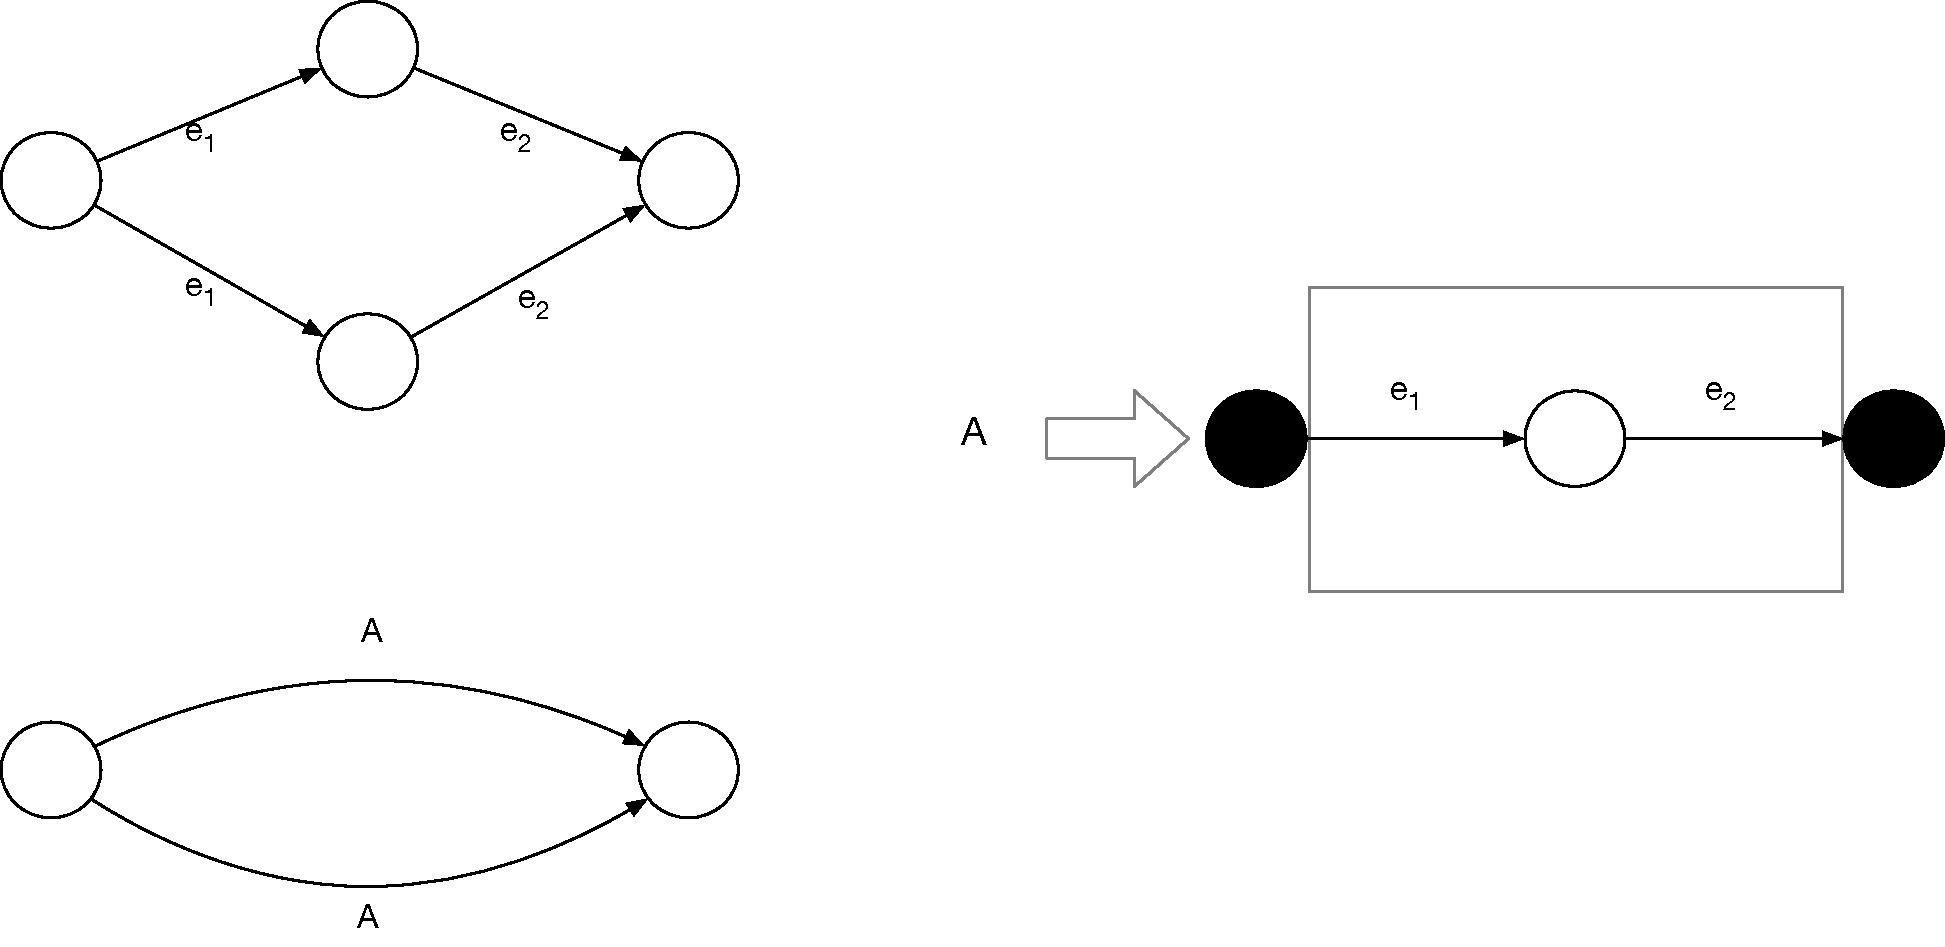
\includegraphics[width=1\textwidth]{img/maneth1}
	\caption{Replacing two different occurrences of the digram A~\cite{maneth}}
	\label{fig:maneth1}
\end{figure}

Apart from~\cite{maneth} there is another approach for a grammar-based compression of graphs by Duerksen~\cite{mattdk} . With this approach the graph is first transformed, as illustrated in Fig.~\ref{fig:transf}. There for each edge a new node (with the former label of the edge) is introduced. Thus two nodes which were previously connected via the edge $e$, are now indirectly connected via the node with the label $e$. The result of the transformation is a graph that only has node labels and no edge labels anymore, which makes compression easier.

\begin{figure}[h]
	\centering
	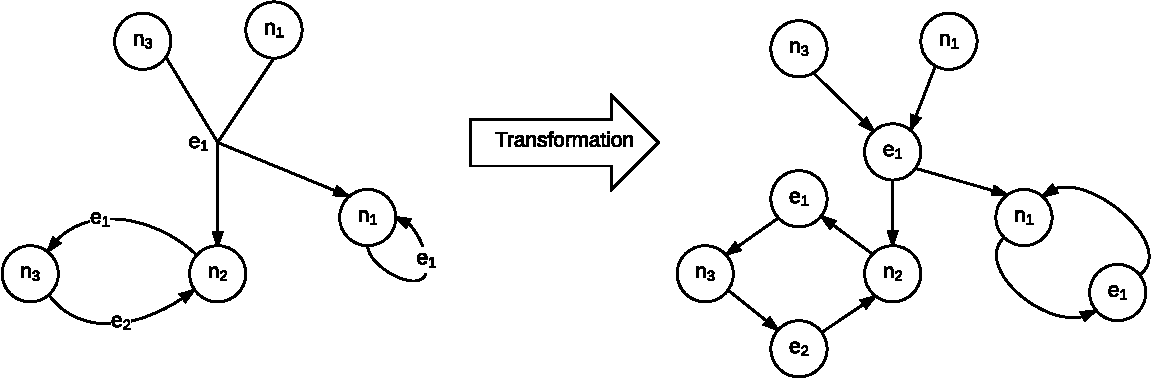
\includegraphics[width=1\textwidth]{img/transf}
	\caption{Transformation of a graph~\cite{mattdk}}
	\label{fig:transf}
\end{figure}

The advantage of the transformation can be seen in Fig.~\ref{fig:digrams_transf}. After the transformation, the four different classes of digrams merge into two different classes. The first of the two different classes is the adjacency digram and the other is the base digram. Adjacency digrams are based on adjacent nodes (digram type 1) or indirectly connected edges (digram type 2). The second type corresponds exactly to the digram of approach~\cite{maneth}. So you can simulate algorithm~\cite{maneth} with algorithm~\cite{mattdk}. The advantage of~\cite{mattdk}, however, is that further digram types are possible. These include base digrams, which are based on the fact that a node has an incident edge with the same label incoming (digram type 4) or outgoing (digram type 3). Such patterns are rather untypical in RDF graphs, but can sometimes occur.

\begin{figure}[h]
	\centering
	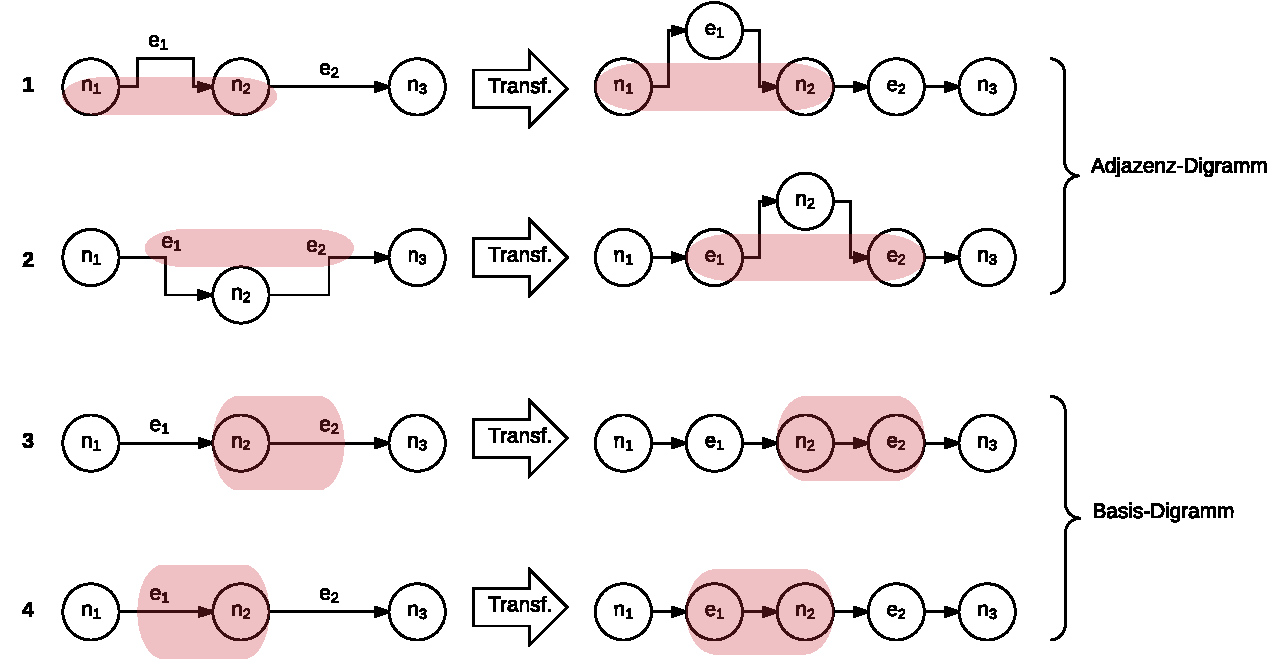
\includegraphics[width=1\textwidth]{img/digrams_transf}
	\caption{Different classes of digrams before and after the transformation from~\cite{mattdk}.}
	\label{fig:digrams_transf}
\end{figure}



\section{This Thesis}

First, it should be investigated which one of the approaches~\cite{maneth} and~\cite{mattdk} works better for RDF graphs.
In~\cite{maneth} a disadvantage is that the nodes have no labels. Therefore we would have to adapt~\cite{maneth} for this thesis. The adaption can be seen in Fig.~\ref{fig:maneth2}. Here the nodes have labels. The digram $A$ now has a parameter $v_1$ which represents the node $v_1$ between the two edges of $A$. Since the different occurrences of $A$ can have different middle nodes, such a parameter is necessary. The two occurrences here each have the middle nodes $v_2$ and $v_4$. Therefore the occurrences are replaced by an edge with the label $A(v_2)$ and $A(v_4)$, respectively.

For~\cite{mattdk} no adaption is necessary.

After the better algorithm has been selected (mostly depending on the compression ratio), the next step is to optimize the algorithm in terms of RDF-specific features. For example, there are symmetrical predicates in RDF, i.e. you can reverse the edge direction (without changing the semantics of the graph) to achieve a possibly higher compression rate.



\begin{figure}[h]
	\centering
	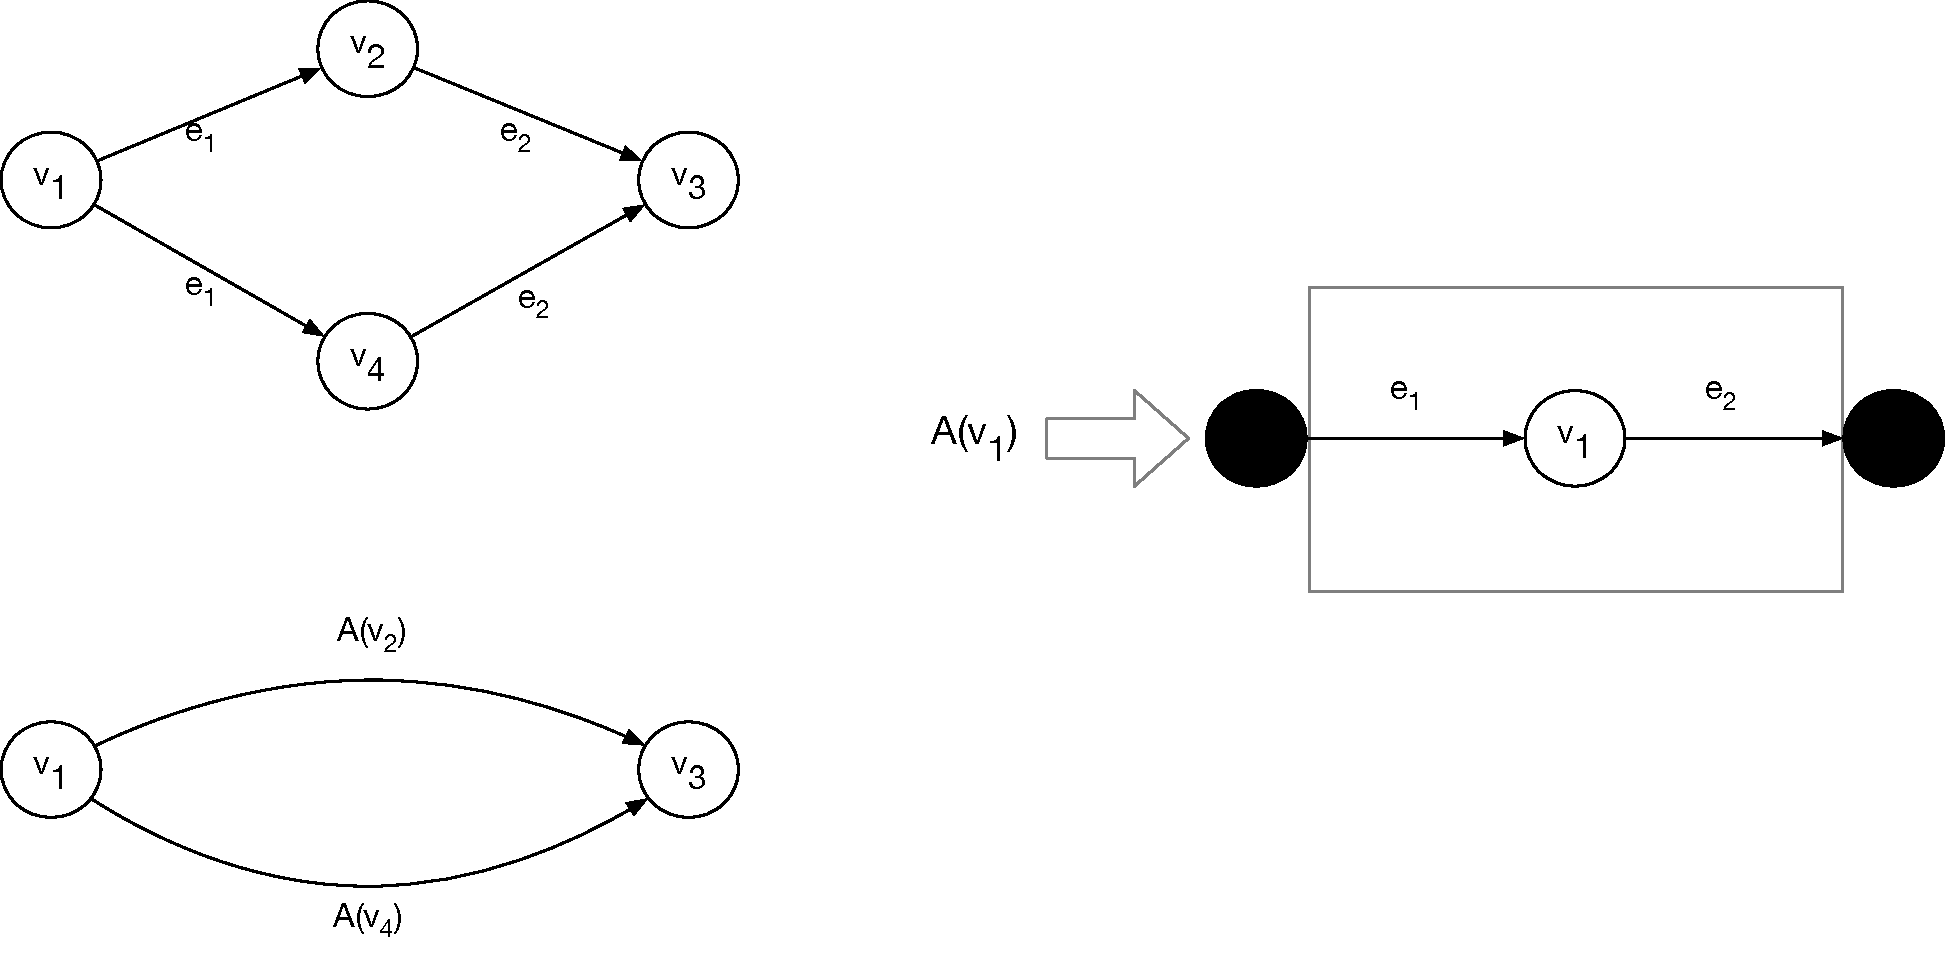
\includegraphics[width=1\textwidth]{img/maneth2}
	\caption{Replacing two different occurrences of the digram A with labeled nodes. Adapted version of~\cite{maneth}.}
	\label{fig:maneth2}
\end{figure}


When the graph has finally been fully compressed by the algorithm (no digrams occur multiple times), the compressed graph must be represented by efficient encoding to minimize memory requirements in order to compare the compression ratio to the one of HDT. The encoding method, of course, depends of the selected compression algorithm. For~\cite{maneth} it would be possible to adapt the already existing method of~\cite{maneth} for the newly introduced parameterization.

For~\cite{mattdk} it yet only exists an encoding method for basis digrams, not for adjacency digrams. The latter one would have to be developed.

A completely different approach would be to pass the compressed graph to the HDT encoding. HDT would have to be adapted to be able to handle digrams. 

The second big question of this thesis is about the speed of queries on the compressed graph. These are so-called SPARQL\footnote{\label{foot:1}https://www.w3.org/TR/rdf-sparql-query/} queries. SPARQL  is a query language for graphs. The queries are based on triples of the form $(S,P,O)$ (Subject, Predicate, Object). One or two components of the triple can be variable (e.g. $(S,?,O)$). Concrete values are then inserted for all non-variable components of the triple. The return value for such a query is then all triples of the graph that correspond to the query pattern.

As already mentioned, a graph compressed by a grammar-based algorithm is still a graph, so it is conceivable that certain types of queries can be executed faster than with a graph compressed by  HDT.

For a sophisticated evaluation real queries made by users are available on the Internet. In the evaluation queries could also be divided in different classes to see which classes are answered faster on which compression algorithm.

In the course of the thesis, an algorithm for answering queries on compressed graphs must firstly be created. There are already approaches in~\cite{maneth} and~\cite{mattdk} for answering queries. It remains to be investigated how well they can be used for SPARQL queries.


\pagebreak
\printbibliography







\end{document}